\documentclass{article}

\usepackage{fullpage}
\usepackage{url}
\usepackage{graphicx}
\usepackage{amsmath}
\usepackage{physics}
\usepackage{mathtools}
\usepackage{bbold}
\usepackage{float}

\usepackage{lmodern}
\usepackage[T1]{fontenc}
\usepackage[fontsize=13.5pt]{fontsize}

\DeclareMathOperator{\erfi}{erfi}
\newcommand{\R}{\ensuremath{\mathbb{R}}}
\newcommand{\C}{\ensuremath{\mathbb{C}}}

\title{Complex Systems Excercise 4}
\author{Idan Stark}
\date{\today}

\begin{document}

\maketitle

\section{Numerics for non-Hermition matrices}
\subsection{Numerical calculations of the Ginibre disk}
To explore the distribution of eigenvalues, we generated $m = 10^4$ square matrices of size $N = 64$. For each item in each matrix, both real and imaginary parts were drawn from a normal distribution $\sim N(0, 0.5)$. Then, using numpy's $np.linalg.eigvals(matrix)$, the eigenvalues were calculated and collected. Figures \ref{fig:part1a} and \ref{fig:part1b} show the distributions of the real and imaginary parts, the distribution of the magnitude and phase, and the scatter plot of all eigenvalues on the complex plane.
\subsection{The scaling of the disk radius with N}
While there are no "maximum" eigenvalues in the complex plane, the maximum magnitude of the eigenvalues matches the radius of the Ginibre disk. The maximum magnitude of eigeanvalues will scale with N similarly to the scaling of the maximum real and imaginary parts, so similar to the way the real maximum eigenvalue scales like the trace, and therefor like $\sqrt{N}$, we can expect that the disk radius will act the same.
\newline
Running the same code, for $m = 10$ matrices for each $N \in [2, 500]$ with jumps of $10$, we can see this scaling in the resulting graph, with $\sqrt{N}$ for comparisent. There is a small error coming from a the proportion constant, so to see that the graphs really scale together it we just plot the graph using logarithmic scales, that way the multiplicative constant becomes an additive constant. Figure \ref{fig:part1c} shows the regular and logarithmic scaled graph.
\begin{figure}[H]
    \centering
    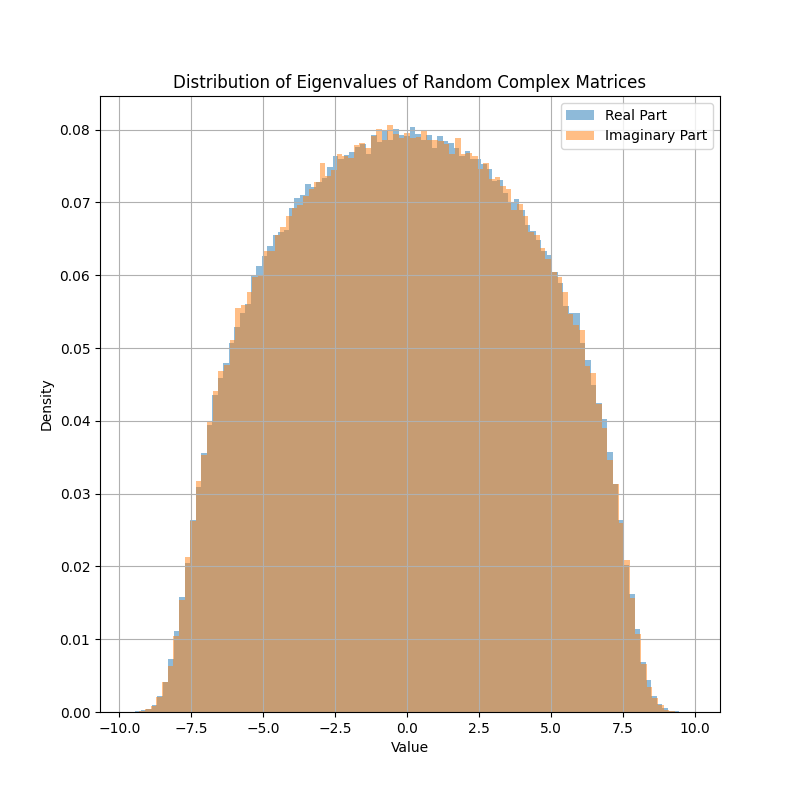
\includegraphics[width=0.4\textwidth]{figures/eigenvalue_distribution.png}
    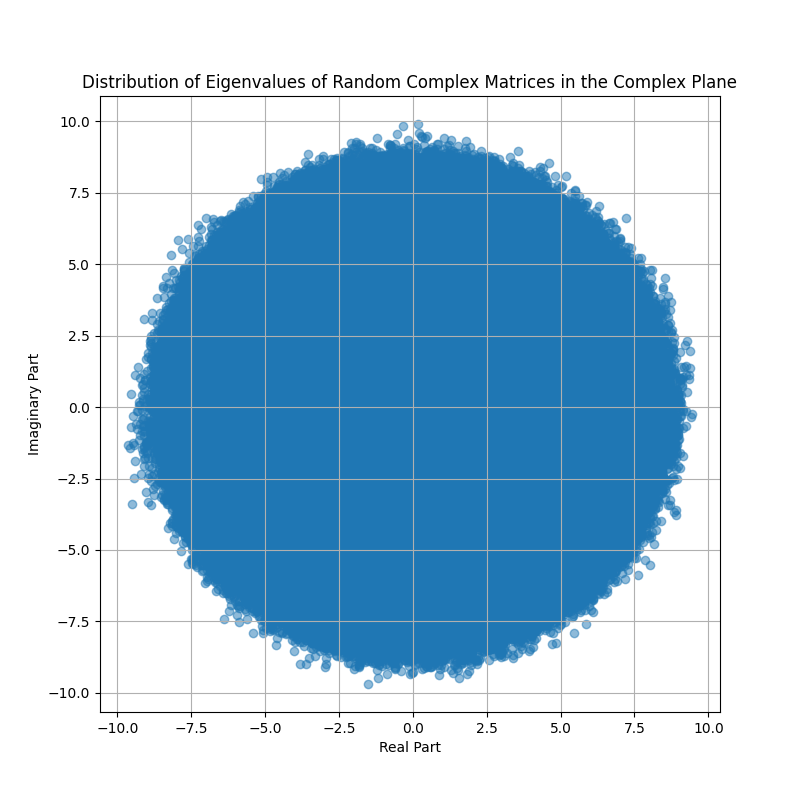
\includegraphics[width=0.4\textwidth]{figures/eigenvalue_complex_plane_distribution.png}
    \caption{Eigeanvalues distributions. The figure on the left shows the distribution of the real and imaginary parts. The values clearly follow the semicircular law. On the right, a scatter plot of the eigenvalues in the complex plane. The Ginibre disk is clearly visible with radius $10$.}
\label{fig:part1a}
\end{figure}
\begin{figure}[H]
    \centering
    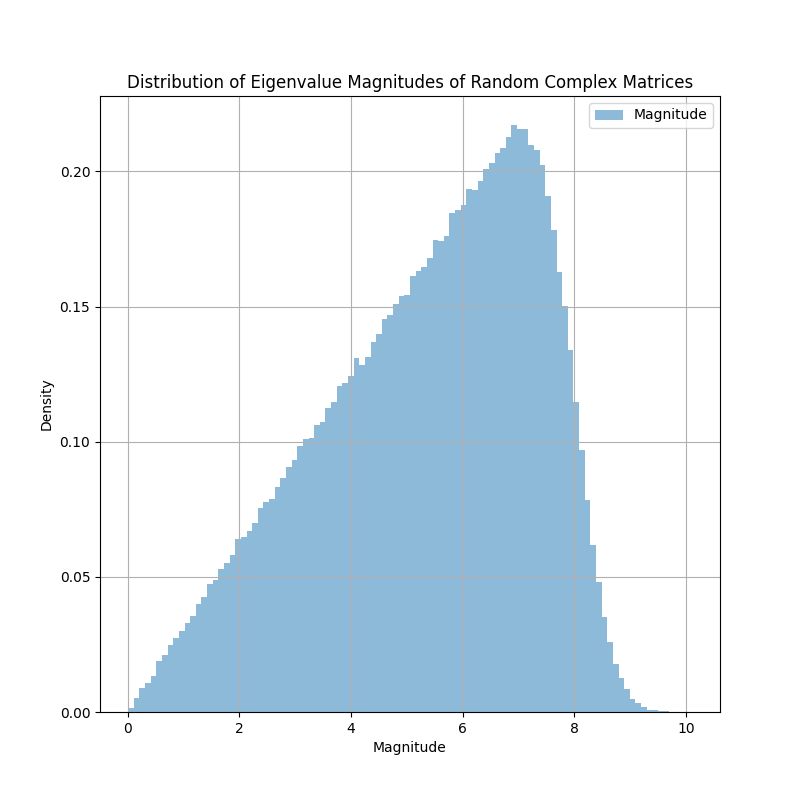
\includegraphics[width=0.4\textwidth]{figures/eigenvalue_magnitude_distribution.png}
    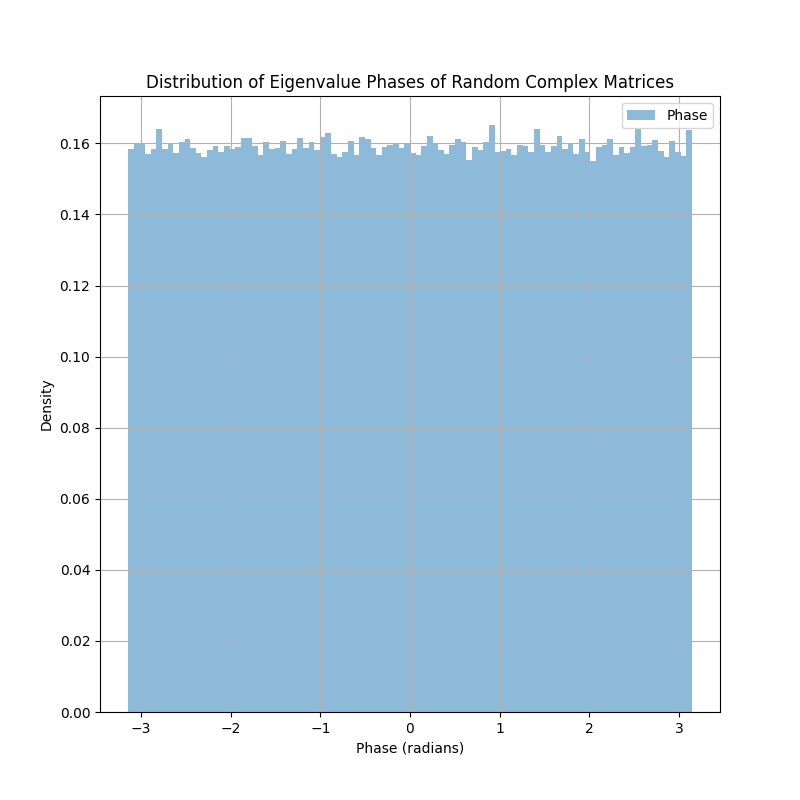
\includegraphics[width=0.4\textwidth]{figures/eigenvalue_phase_distribution.png}
    \caption{The magnitude and phase of the complex eigenvalues. The graph on the left shows the radial distribution of the eigenvalues while the graph on the right shows the phase distribution. It's clear that the phase is uniformly distributed while the radial part is linearly distributed, fitting the Jacobean. At the edge of the radial distribution the edge of the semi-circle law is visible.}
\label{fig:part1b}
\end{figure}
\begin{figure}[H]
    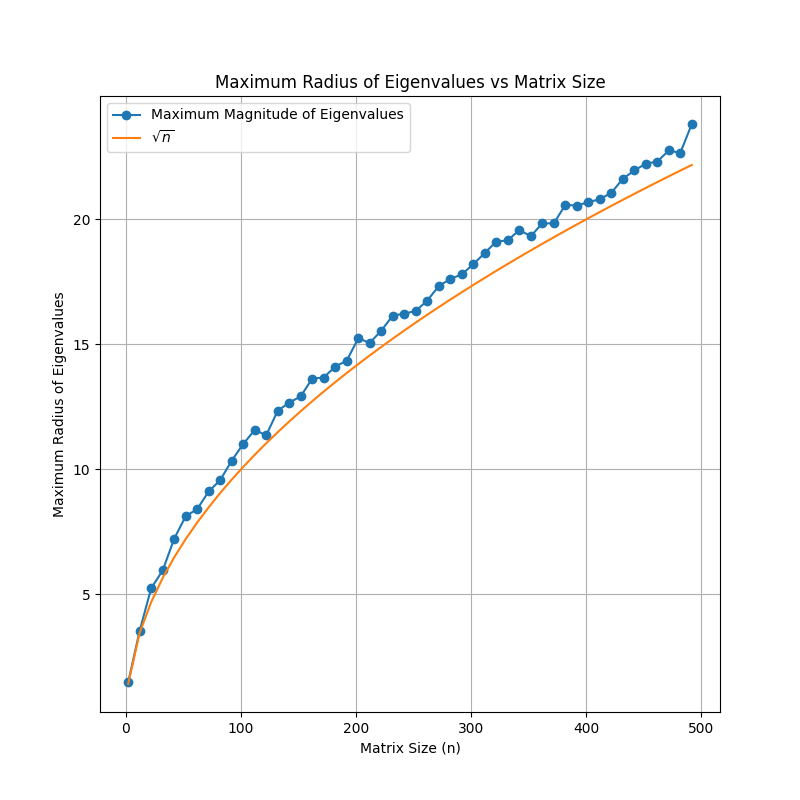
\includegraphics[width=0.5\textwidth]{figures/radius_vs_n.png}
    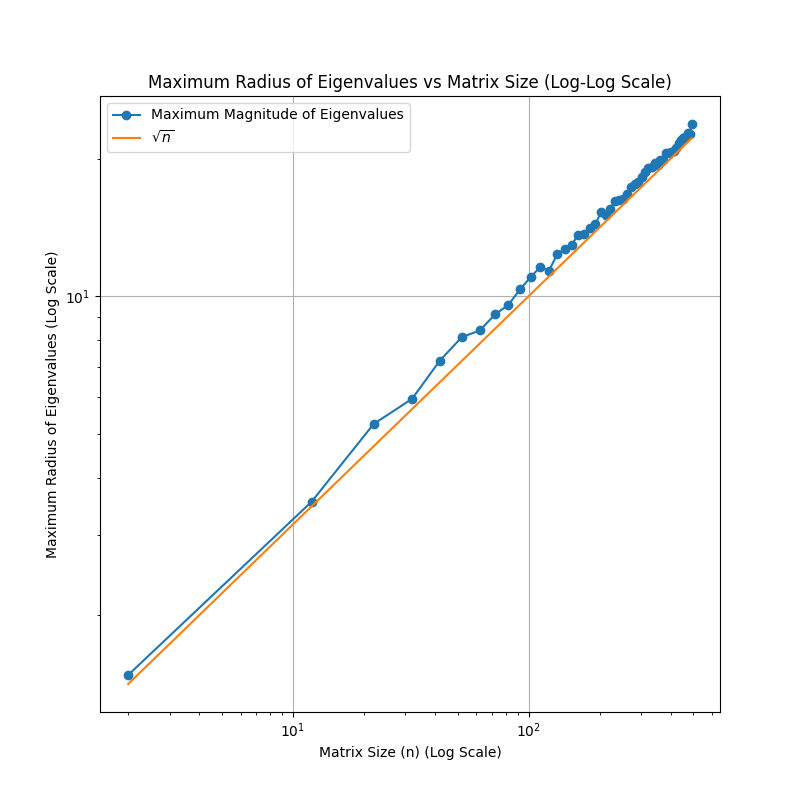
\includegraphics[width=0.5\textwidth]{figures/radius_vs_n_loglog.png}
    \caption{Graphs comparing the maximal magnitude of the eigenvalues as a function of matrix size. The graph on the left shows the regular scale while the graph on the right shows the logarithmic scale.}
\label{fig:part1c}
\end{figure}
\subsection{Level repulsion}
Like in other matrix ensembles, the probability to get close eigenvalues will be lowered by level repulsion. Unlike in the cases of GOE and GUE, the eigenvalues are not real, and thus don't have any ordering. So, we must define the distance of the eigenvalues in a way that represents the geometry of the complex plane. The easist way is to define the distance between two eigenvalues as the norm of their difference:
\begin{equation}
    d_{i,j} = \left|\lambda_i - \lambda_j\right|
\end{equation}
In GOE and GUE, we took the distance between every two consequtive eigenvalues after sorting them. The equivilant here is a bit more complex (see what I did there?). We need to select which neighboor will be taken as the "consequtive" eigenvalue.
\newline
We will just go around this problem by only considering $N = 2$ matrices. In the previous section we saw that the eigenvalue distribution is the same regardless of $N$ chosen, and scales with $\sqrt{N}$. We can assume then, that if the distribution of (noramlized) eigenvalues has no dependence on $N$, so does the distribution of whatever geometrically appropriate distance measure we choose.
\newline
We expect that we again get distribution similar to the other two ensembles:
\begin{equation}
    p(s) = A s^\beta e^{-B s^2} 
\end{equation}
Where $A$ and $B$ are determinted by the normalization and centralization conditions:
\begin{equation}
    \int_0^\infty p(s) ds = 1 \qquad \langle s \rangle = \int_0^\infty sp(s) ds = 1
\end{equation}
In GOE we use $\beta = 1$ and in GUE we use $\beta = 2$, coming from the two degrees of freedom in the complex value of the off diagonal items. In Ginibre, we assume that not only do we get the two degrees of freedom from the complex value of the off diagonal items, but also we get an additional $+1$ to the power, coming from the fact that the eigenvalues themselves are complex, giving an additional degree of freedom to the distance defition. All in all, we can expect $\beta = 3$. The normalization and centralization then give us the distribution:
\begin{equation}
    p(\Delta \lambda) = \frac{81\pi^2}{128} \Delta \lambda^3 e^{-\frac{9\pi}{16}\Delta \lambda^2}
\end{equation}
% \newline
% At this point I think it would be interesting to actually calculate $\Delta \lambda$ from the $2 \times 2$ matrix, as we did in class. Just to make sure we didn't miss anything. Since it's general and non-hermitian, we can write it as:
% \begin{equation}
%     A = \begin{pmatrix}
%         a & b \\ d & c
%     \end{pmatrix}
% \end{equation}
% The eigenvalues follow:
% \begin{equation}
%     (a - \lambda)(c - \lambda) - bd = 0
% \end{equation}
% \begin{equation}
%     \lambda^2 - (a + c)\lambda + ac - bd = 0
% \end{equation}
% \begin{equation}
%     \lambda = \frac{a + c}{2} \pm \frac{1}{2}\sqrt{(a + c)^2 - 4(ac - bd)}
% \end{equation}
% \begin{equation}
%     \Delta \lambda = \sqrt{(a + c)^2 - 4(ac - bd)} = \sqrt{(a - c)^2 +4bd}
% \end{equation}
% To make at least some of the integration simpler, we can define:
% \begin{equation}
%     \xi_1 = a - c \qquad \xi_2 = b + d \qquad \xi_3 = b - d
% \end{equation}
% Which wille give:
% \begin{equation}
%     \Delta \lambda = \sqrt{\xi_1^2 + \xi_2^2 - \xi_3^2}
% \end{equation}
% Obviously the variance of each of these variables is $2\sigma^2 = 0.5$ and their joint probability distribution is a 3D gaussian:
% \begin{equation}
%     p(\xi_1,\xi_2,\xi_3) \propto e^{-\left(\xi_1^2 + \xi_2^2 + \xi_3^2\right)} \propto s^2 e^{-s^2}
% \end{equation}
% Where $s = \xi_1^2 + \xi_2^2 + \xi_3^2$ and we added the Jacobean.
% \begin{equation}
% \begin{gathered}
%     a^2 + b^2 + c^2 + d^2 = 2x^2 + 2y^2 + (b + d)^2 - 2(ac) - 2t^2
%     \\
%     \sqrt{(a + c)^2 - 4(ac - bd)} = \sqrt{4x^2 - 4t^2}
% \end{gathered}
% \end{equation}
\newline
Running the simulation with the same parameters as in the previous sections, taking only matrices with $N = 2$ and appropriatly increasing the population to $10^6$, we get a perfect match to this distribution, as visible in Figure \ref{fig:level-spacing}.
\begin{figure}[H]
    \centering
    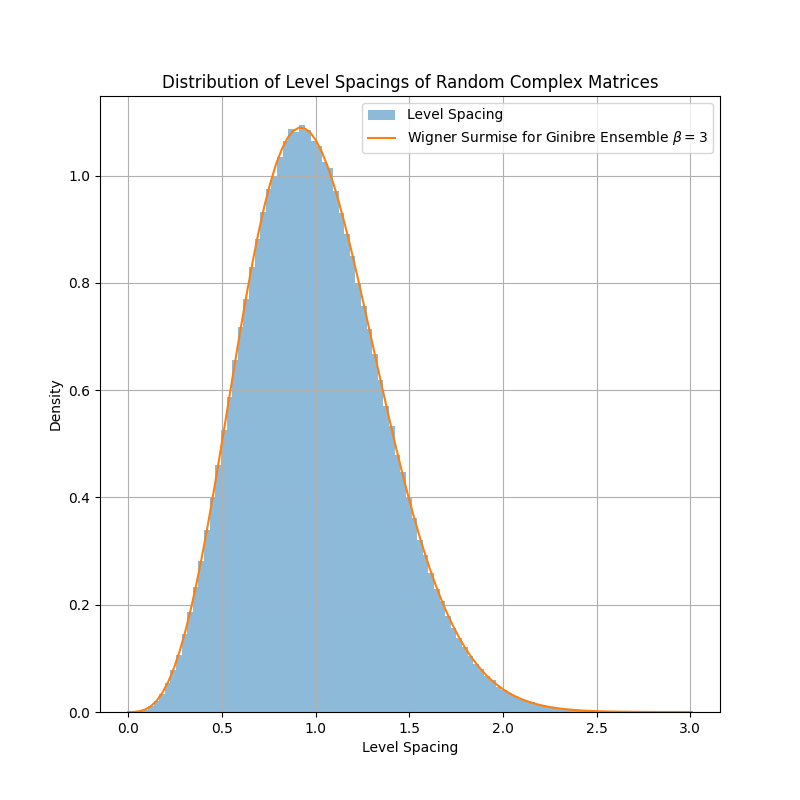
\includegraphics[width=0.8\textwidth]{figures/level_spacings_distribution.png}
    \caption{The random sampling of $\Delta \lambda$ for $N = 2$ matrices. The orange line represents the Winger Surmise for $\beta = 3$.}
    \label{fig:level-spacing}
\end{figure}

\newpage
\section{Black swans}
\subsection{The sum of $n$ variables}
We consider $n$ i.i.d positive random variables $X_1, \dots, X_n$ from a distribution with the tail (for large x):
\begin{equation}
    p(x) \propto x^{-(1 + \mu)} \qquad 0 < \mu < 2
\end{equation}
% TODO finish this.
Using a Taburian theorem for the power law, for small $\omega$, we get that the Characteristic function is:
\begin{equation}
    \phi(\omega) \propto 1 - A |\omega|^\mu + \cdots
\end{equation}
Now, the joint probability distribution their sum follow convolution, and so its Characteristic function is simply a product:
\begin{equation}
    \phi_n(\omega) \propto (1 - A |\omega|^\mu)^n \approx 1 - nA\omega^\mu 
\end{equation}
Where we used a simple Newton's binomial and again ignored anything above first order in $\omega^\mu$. Performing the inverse Fourier transform:
\begin{equation}
    p_n^{sum}(x) \propto nx^{-(1 + \mu)}
\end{equation}
\subsection{The maximum out of $n$ variables}
As we saw in class, the probability distribution of exterme values follow a simple multiplicative pattern (we require all values to be below some maximal value, which is a multiplication of their CDF). The CDF of a single variable is:
\begin{equation}
    p(X < x) = 1 - p(X > x) = 1 - \int_x^\infty t^{-(1 + \mu)}dt = 1 - \frac{x^{-\mu}}{1 + \mu}
\end{equation}
So:
\begin{equation}
    p_n(X_i < x) = p^n(X < x) = \left[1 - \frac{x^{-\mu}}{1 + \mu}\right]^n \approx 1 - \frac{n}{1 + \mu}x^{-\mu}
\end{equation}
And so:
\begin{equation}
    p_n^{max}(x) = \frac{d}{dx}p_n(X_i < x) = n x^{-(1 + \mu)}
\end{equation}
\subsection{Single big jump}
We can see that both distribution are of the same order of magnitude in both $n$ and $x$, meaning that the probability of getting a maximum item at the same order of magnitude as the same is 1.
\subsection{Numerical results}
In this section we show this result numerically. We take the distribution
\begin{equation}
    p(x) = \mu (1 + x)^{-(1 + \mu)}
\end{equation}
Since for large values of $x$ this distribution has a heavy tail where $x \gg 1$. This is also simple because we can use numpy's built in pareto function. We run $10^6$ iteractions with $n = 30$ for each value $\mu = 0.5, 1, 1.5$. Then, for each value of $\mu$, we take only the top sums, taking larger and larger percentile cutoffs, running from $0.9$ to $0.999$, and plotting the percentile taken vs the ratio of the maximum and the sum. It can be seen in the graph in figure \ref{fig:part2}, that the closer the sum is to being the maximum sum, the larger portion of it is taken by the maximum value.
\begin{figure}[H]
    \centering
    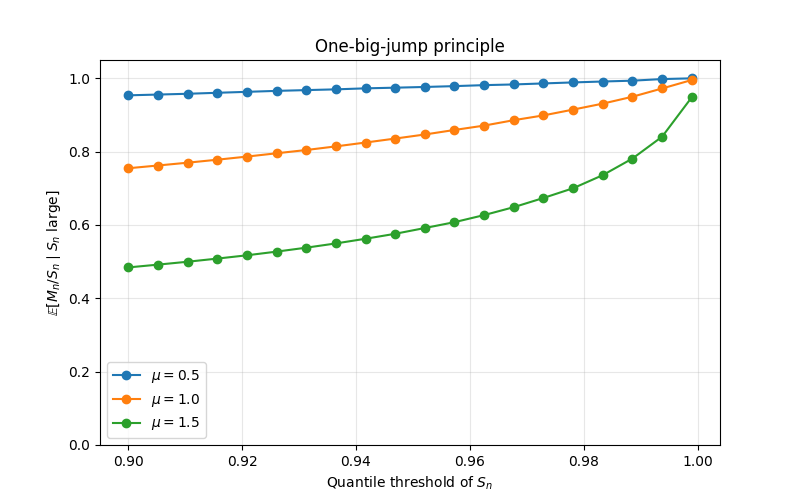
\includegraphics[width=0.8\textwidth]{figures/part2.png}
    \caption{The part of the sum taken by the largest value, averaged over all iteraction where the sum is above a quantile, as a function of the quantile threshold. It can be seen that the larger the quantile, i.e. the more extreme the sums are, the more they are domindated by a single value.}
\label{fig:part2}
\end{figure}
\end{document}